% Options for packages loaded elsewhere
\PassOptionsToPackage{unicode}{hyperref}
\PassOptionsToPackage{hyphens}{url}
%
\documentclass[
]{article}
\usepackage{amsmath,amssymb}
\usepackage{lmodern}
\usepackage{iftex}
\ifPDFTeX
  \usepackage[T1]{fontenc}
  \usepackage[utf8]{inputenc}
  \usepackage{textcomp} % provide euro and other symbols
\else % if luatex or xetex
  \usepackage{unicode-math}
  \defaultfontfeatures{Scale=MatchLowercase}
  \defaultfontfeatures[\rmfamily]{Ligatures=TeX,Scale=1}
\fi
% Use upquote if available, for straight quotes in verbatim environments
\IfFileExists{upquote.sty}{\usepackage{upquote}}{}
\IfFileExists{microtype.sty}{% use microtype if available
  \usepackage[]{microtype}
  \UseMicrotypeSet[protrusion]{basicmath} % disable protrusion for tt fonts
}{}
\makeatletter
\@ifundefined{KOMAClassName}{% if non-KOMA class
  \IfFileExists{parskip.sty}{%
    \usepackage{parskip}
  }{% else
    \setlength{\parindent}{0pt}
    \setlength{\parskip}{6pt plus 2pt minus 1pt}}
}{% if KOMA class
  \KOMAoptions{parskip=half}}
\makeatother
\usepackage{xcolor}
\IfFileExists{xurl.sty}{\usepackage{xurl}}{} % add URL line breaks if available
\IfFileExists{bookmark.sty}{\usepackage{bookmark}}{\usepackage{hyperref}}
\hypersetup{
  pdftitle={2021-01-25\_lacre},
  pdfauthor={Gonzalo García-Castro},
  hidelinks,
  pdfcreator={LaTeX via pandoc}}
\urlstyle{same} % disable monospaced font for URLs
\usepackage[margin=1in]{geometry}
\usepackage{color}
\usepackage{fancyvrb}
\newcommand{\VerbBar}{|}
\newcommand{\VERB}{\Verb[commandchars=\\\{\}]}
\DefineVerbatimEnvironment{Highlighting}{Verbatim}{commandchars=\\\{\}}
% Add ',fontsize=\small' for more characters per line
\usepackage{framed}
\definecolor{shadecolor}{RGB}{248,248,248}
\newenvironment{Shaded}{\begin{snugshade}}{\end{snugshade}}
\newcommand{\AlertTok}[1]{\textcolor[rgb]{0.94,0.16,0.16}{#1}}
\newcommand{\AnnotationTok}[1]{\textcolor[rgb]{0.56,0.35,0.01}{\textbf{\textit{#1}}}}
\newcommand{\AttributeTok}[1]{\textcolor[rgb]{0.77,0.63,0.00}{#1}}
\newcommand{\BaseNTok}[1]{\textcolor[rgb]{0.00,0.00,0.81}{#1}}
\newcommand{\BuiltInTok}[1]{#1}
\newcommand{\CharTok}[1]{\textcolor[rgb]{0.31,0.60,0.02}{#1}}
\newcommand{\CommentTok}[1]{\textcolor[rgb]{0.56,0.35,0.01}{\textit{#1}}}
\newcommand{\CommentVarTok}[1]{\textcolor[rgb]{0.56,0.35,0.01}{\textbf{\textit{#1}}}}
\newcommand{\ConstantTok}[1]{\textcolor[rgb]{0.00,0.00,0.00}{#1}}
\newcommand{\ControlFlowTok}[1]{\textcolor[rgb]{0.13,0.29,0.53}{\textbf{#1}}}
\newcommand{\DataTypeTok}[1]{\textcolor[rgb]{0.13,0.29,0.53}{#1}}
\newcommand{\DecValTok}[1]{\textcolor[rgb]{0.00,0.00,0.81}{#1}}
\newcommand{\DocumentationTok}[1]{\textcolor[rgb]{0.56,0.35,0.01}{\textbf{\textit{#1}}}}
\newcommand{\ErrorTok}[1]{\textcolor[rgb]{0.64,0.00,0.00}{\textbf{#1}}}
\newcommand{\ExtensionTok}[1]{#1}
\newcommand{\FloatTok}[1]{\textcolor[rgb]{0.00,0.00,0.81}{#1}}
\newcommand{\FunctionTok}[1]{\textcolor[rgb]{0.00,0.00,0.00}{#1}}
\newcommand{\ImportTok}[1]{#1}
\newcommand{\InformationTok}[1]{\textcolor[rgb]{0.56,0.35,0.01}{\textbf{\textit{#1}}}}
\newcommand{\KeywordTok}[1]{\textcolor[rgb]{0.13,0.29,0.53}{\textbf{#1}}}
\newcommand{\NormalTok}[1]{#1}
\newcommand{\OperatorTok}[1]{\textcolor[rgb]{0.81,0.36,0.00}{\textbf{#1}}}
\newcommand{\OtherTok}[1]{\textcolor[rgb]{0.56,0.35,0.01}{#1}}
\newcommand{\PreprocessorTok}[1]{\textcolor[rgb]{0.56,0.35,0.01}{\textit{#1}}}
\newcommand{\RegionMarkerTok}[1]{#1}
\newcommand{\SpecialCharTok}[1]{\textcolor[rgb]{0.00,0.00,0.00}{#1}}
\newcommand{\SpecialStringTok}[1]{\textcolor[rgb]{0.31,0.60,0.02}{#1}}
\newcommand{\StringTok}[1]{\textcolor[rgb]{0.31,0.60,0.02}{#1}}
\newcommand{\VariableTok}[1]{\textcolor[rgb]{0.00,0.00,0.00}{#1}}
\newcommand{\VerbatimStringTok}[1]{\textcolor[rgb]{0.31,0.60,0.02}{#1}}
\newcommand{\WarningTok}[1]{\textcolor[rgb]{0.56,0.35,0.01}{\textbf{\textit{#1}}}}
\usepackage{graphicx}
\makeatletter
\def\maxwidth{\ifdim\Gin@nat@width>\linewidth\linewidth\else\Gin@nat@width\fi}
\def\maxheight{\ifdim\Gin@nat@height>\textheight\textheight\else\Gin@nat@height\fi}
\makeatother
% Scale images if necessary, so that they will not overflow the page
% margins by default, and it is still possible to overwrite the defaults
% using explicit options in \includegraphics[width, height, ...]{}
\setkeys{Gin}{width=\maxwidth,height=\maxheight,keepaspectratio}
% Set default figure placement to htbp
\makeatletter
\def\fps@figure{htbp}
\makeatother
\setlength{\emergencystretch}{3em} % prevent overfull lines
\providecommand{\tightlist}{%
  \setlength{\itemsep}{0pt}\setlength{\parskip}{0pt}}
\setcounter{secnumdepth}{-\maxdimen} % remove section numbering
\usepackage{amsmath}
\usepackage{booktabs}
\usepackage{caption}
\usepackage{longtable}
\ifLuaTeX
  \usepackage{selnolig}  % disable illegal ligatures
\fi
\newlength{\cslhangindent}
\setlength{\cslhangindent}{1.5em}
\newlength{\csllabelwidth}
\setlength{\csllabelwidth}{3em}
\newenvironment{CSLReferences}[2] % #1 hanging-ident, #2 entry spacing
 {% don't indent paragraphs
  \setlength{\parindent}{0pt}
  % turn on hanging indent if param 1 is 1
  \ifodd #1 \everypar{\setlength{\hangindent}{\cslhangindent}}\ignorespaces\fi
  % set entry spacing
  \ifnum #2 > 0
  \setlength{\parskip}{#2\baselineskip}
  \fi
 }%
 {}
\usepackage{calc}
\newcommand{\CSLBlock}[1]{#1\hfill\break}
\newcommand{\CSLLeftMargin}[1]{\parbox[t]{\csllabelwidth}{#1}}
\newcommand{\CSLRightInline}[1]{\parbox[t]{\linewidth - \csllabelwidth}{#1}\break}
\newcommand{\CSLIndent}[1]{\hspace{\cslhangindent}#1}

\title{2021-01-25\_lacre}
\author{Gonzalo García-Castro}
\date{10/11/2021}

\begin{document}
\maketitle

\hypertarget{background}{%
\subsection{Background}\label{background}}

Infants learning two languages face the challenge of having to learn two
distinct sets of words. Some of the words across both languages refer to
similar concepts: for instance, \emph{chair} and \emph{silla} (in
Spanish). These pairs of words are called \emph{translation
equivalents}. Sometimes, translation equivalents also overlap in form,
frequently due to their shared etymological origin. These form-similar
translation equivalents, such as \emph{boot} and \emph{bota} (in
Spanish), are referred to as \emph{cognates}.

There is extensive literature on how cognateness impacts the dynamics of
lexical access during words comprehension and production. One of its
main findings is that bilinguals process cognates (such as \emph{boot}
and \emph{bota}) more differently than non-cognates (such as
\emph{chair} and \emph{silla}). For instance, Costa, Caramazza, and
Sebastian-Galles (2000) asked Spanish-Catalan bilinguals to name a
series of familiar pictures in Spanish. Part of the pictures referred to
objects whose labels in Spanish and Catalan were cognates, whereas the
other pictures referred to non-cognates. On average, participants named
cognate pictures faster than non-cognate pictures. This effect was
independent of lexical frequency and, critically, was not observed when
Spanish monolinguals performed the same task. This suggests that
bilinguals activated labels in both languages, and that their phonology
interacted to facilitate naming.

Later studies provided evidence that the locus of this facilitation
effect was at the lexical level, and not just at the articulatory level
{[}reference needed here{]}: this effect has also been reported during
comprehension, at both the visual-orthographic and the
auditory-phonology modalities) (e.g., Thierry and Wu 2007). Overall,
these findings have led researchers to hypothesise that lexical access
is language-non selective, that is, bilinguals activate lexical
representations in both languages in parallel during comprehension and
production, based on their semantic and phonological overlap.

This cross-talk between languages has also been suggested to be present
in children's and toddlers' lexicon (Von Holzen and Mani 2012; Bosma and
Nota 2020), but it is still unclear how it impacts the trajectories of
language acquisition at these early ages. In this study we sought to
investigate the developmental trajectories of lexical access in a cohort
of Catalan-Spanish and English-Spanish bilinguals.

To do this, we used an adaptation of Mani and Plunkett (2010)'s priming
paradigm. This paradigm consists of a spoken word recognition task in
which participants are first presented with a picture in silence in the
centre of the screen for 1.5 seconds. Then, two other pictures are
presented side-by-side during 2 seconds, and one of them is named. The
other is not. Looking times to the target picture are recorded from name
onset. From now on, I will refer to the silent picture presented first
as the \emph{prime}, to the named picture as the \emph{target}, and to
the non-named picture presented next to the target as \emph{distractor}.

In their experiment, Mani and Plunkett manipulated the phonological
overlap between the prime label and the target label: in some trials,
both labels shared phonological onset (\emph{bee}-\emph{ball}), whereas
in other trials they did not share phonological onset
(\emph{cow}-\emph{book}). In all trials, the distractor label did not
share onset with either of the prime or target labels (e.g.,
\emph{teeth}). The authors registered 18 month-old participants' looking
preference for the target object after name onset, as a proxy of word
recognition, and found that target preference was stronger after a
phonologically related prime than after a phonologically unrelated
prime. There results have three main implications:

\begin{enumerate}
\def\labelenumi{\arabic{enumi})}
\tightlist
\item
  Phonologically related prime pictures facilitated target recognition
\item
  This is only possible if participants lexicalised the prime pictures,
  even though this picture was presented in silence
\item
  The label participants generated upon prime picture presentation was
  phonologically detailed, and this phonological form interacted with
  the auditory recognition of a subsequently presented word
\end{enumerate}

In a subsequent study, the authors found the inverse effect in 24
month-old toddlers: target looking preference was weaker after a
phonologically related prime picture compared to after an unrelated one
(Mani and Plunkett 2011). The authors suggested that the change in the
direction of the effect observed between 18 and 24 month-old
participants was due to the increment in vocabulary size and the
establishment of (inhibitory) links between phonologically related
lexical entries that might have occurred between both ages. Supporting
this account, the inhibition effect they reported was stronger as the
number of phonological neighbours of the target increased: the
recognition of words surrounded by more phonologically related
neighbours suffered the most from the priming effect.

We adapted this paradigm to test the language-non selectivity account in
bilingual toddlers. Following Mani \& Plunkett's original
implementation, In our task half of the prime-target pairs in the trial
lists shared phonological onset, and the other half did not share
phonological onset. We added a novel manipulation: half of the primes in
the phonologically related condition were cognates and the other half
were non-cognates. We classified two translation equivalents as cognates
if they shared phonological onset. Here is an illustration of each trial
type:

\captionsetup[table]{labelformat=empty,skip=1pt}
\begin{longtable}{llll}
\toprule
Prime type & Prime & Target & Distractor \\ 
\midrule
Cognate (N = 8) & flower (flor) & fork & balloon \\ 
Non-cognate (N = 8) & tree (árbol) & truck & phone \\ 
Unrelated (N = 16) & penguin (pingüino) & table & shoe \\ 
\bottomrule
\end{longtable}

This is what a trial looks like {[}see figure below{]}:

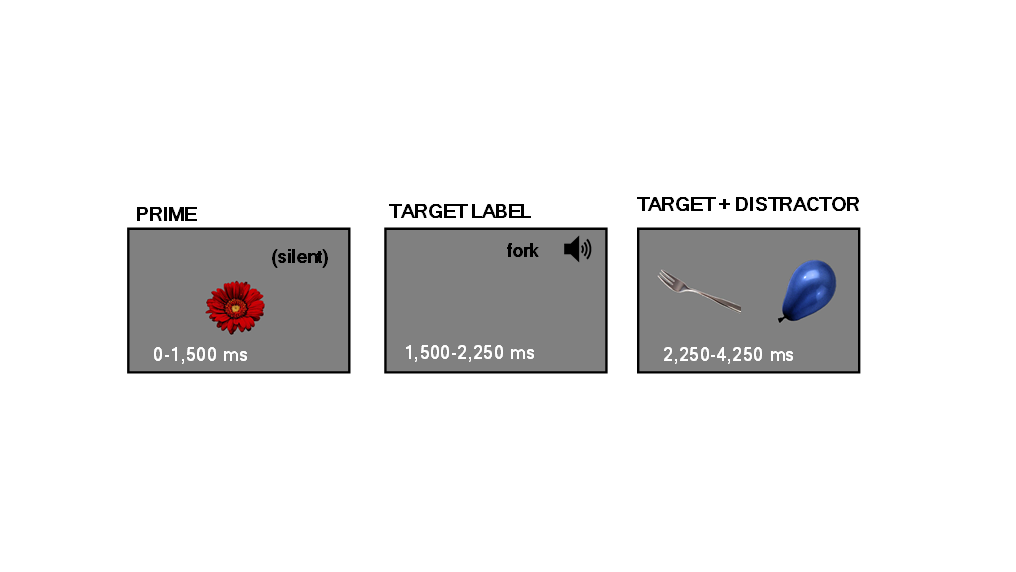
\includegraphics{img/task.png}

\hypertarget{hypotheses}{%
\subsection{Hypotheses}\label{hypotheses}}

If participants lexicalise the prime pictures in a language-non
selective way, they should generate two labels upon prime picture
presentation: one in each language. Therefore, if lexical access is
language non-selective, in cognate trials two prime labels should
interfere with target recognition (since both prime labels share onset
with the target). In non-cognate trials, only one prime label should
interfere with the target. Finally, in unrelated trials no prime labels
should interfere with the target. As a result, we expect bilingual
participants' target looking preference to be weaker in cognate trials
than in non-cognate trials, and in cognate and non-cognate trials than
in unrelated trials.

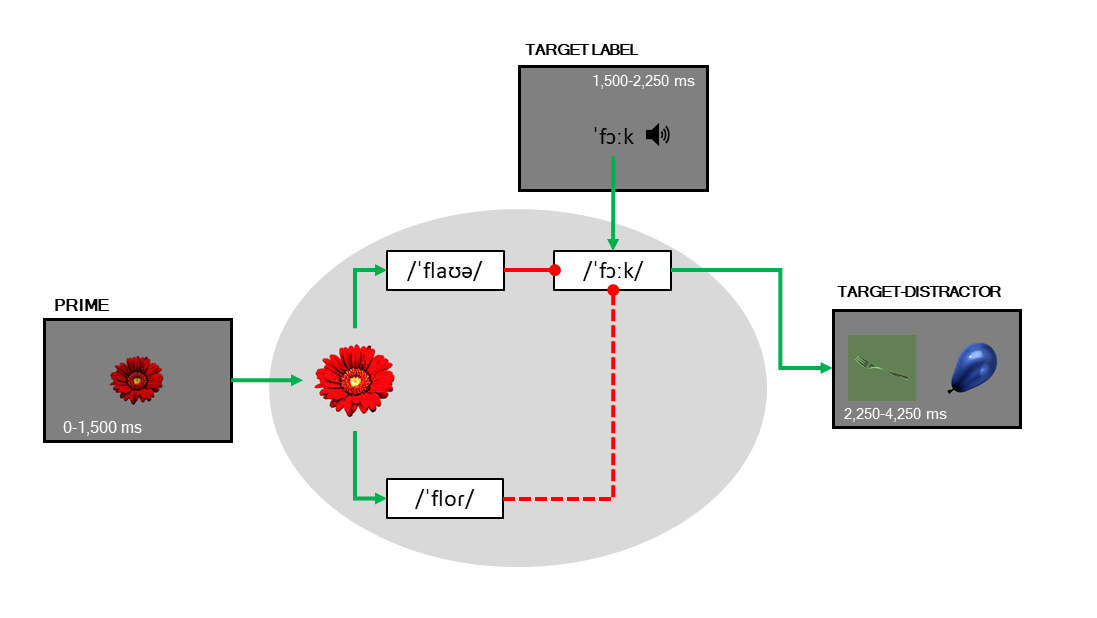
\includegraphics{img/diagram.png}

We also collected data from same-aged monolingual participants as a
control group: in this group we also expect to find weaker target
looking in cognate and non-cognate trials, compared to unrelated trials,
but no differences between cognate and non-cognate trials (these
participants should be insensitive to the cognate status of the primes).

\hypertarget{participants}{%
\subsection{Participants}\label{participants}}

We planned to collect data from participants learning English and/or
Spanish in Oxford, and from participants learning Catalan and/or Spanish
in Barcelona. Due to limitations imposed by the pandemic and lockdown,
data collection in Oxford was severely interrupted, so I will present
preliminary data from participants tested in Barcelona exclusively.

We tested participants at three age points: 21, 25, and 30 months, to
explore their trajectories of lexical access through these sensitive
ages in which participants' vocabulary size is growing a full speed
{[}Reference here.{]}

We classified participants as monolinguals or bilinguals by estimating
their overall exposure to each of their languages using Bosch and
Sebastián-Gallés (2001). Following the consensus reached by the
ManyBabies consortium (Byers-Heinlein et al. 2021), participants exposed
to any languages more than 80\% of the time were classified as
monolinguals. Otherwise, participants were classified as bilinguals.
Participants exposed more than 10\% to a third language or a language
other than Catalan and Spanish (in Barcelona) or English and Spanish (in
Oxford) were excluded from data analysis.

This is how testing sessions are distributed across ages and language
profiles:

\captionsetup[table]{labelformat=empty,skip=1pt}
\begin{longtable}{llrrrr}
\toprule
 & Testing language & 21 months & 25 months & 30 months & N \\ 
\midrule
\multicolumn{1}{l}{Bilingual} \\ 
\midrule
 & Catalan & 13 & 7 & 8 & 28 \\ 
 & Spanish & 12 & 7 & 11 & 30 \\ 
\midrule
\multicolumn{1}{l}{Monolingual} \\ 
\midrule
 & Catalan & 26 & 20 & 13 & 59 \\ 
 & Spanish & 18 & 9 & 12 & 39 \\ 
\bottomrule
\end{longtable}

These 156 testing sessions correspond to 106 distinct participants. Of
these participants, 1, 64 only participated once (I will refer top these
participants as cross-sectional participants), 2, 34 participated twice,
and 3, 8 participated three times.

\hypertarget{data-analysis}{%
\subsection{Data analysis}\label{data-analysis}}

\begin{Shaded}
\begin{Highlighting}[]
\NormalTok{n\_obs }\OtherTok{\textless{}{-}} \FunctionTok{nrow}\NormalTok{(fit}\SpecialCharTok{$}\NormalTok{data)}

\NormalTok{n\_trials\_total }\OtherTok{\textless{}{-}} \FunctionTok{distinct}\NormalTok{(fit}\SpecialCharTok{$}\NormalTok{data, participant, target, trial\_type) }\SpecialCharTok{\%\textgreater{}\%} 
    \FunctionTok{count}\NormalTok{() }\SpecialCharTok{\%\textgreater{}\%} 
    \FunctionTok{pull}\NormalTok{(n)}

\NormalTok{n\_trials }\OtherTok{\textless{}{-}} \FunctionTok{distinct}\NormalTok{(gaze, participant, trial, trial\_type) }\SpecialCharTok{\%\textgreater{}\%} 
    \FunctionTok{count}\NormalTok{(trial\_type) }\SpecialCharTok{\%\textgreater{}\%} 
    \FunctionTok{pull}\NormalTok{(n, }\AttributeTok{name =}\NormalTok{ trial\_type)}
\end{Highlighting}
\end{Shaded}

In each testing session, participants were presented with 32 trials (8
cognate, 8 non-cognate and 16 unrelated). In each trial, we used an
eye-tracker to register participants' looking time to the target
picture. We delimited a time window of interest between 250 ms after the
target onset and 150 ms before the target offset. This resulted in a
1,500 ms long time window. We divided this time window into 15 time bins
of 100 ms each, and calculated the adjusted logit of the samples in
which participants' gaze was located in the target coordinates, out of
the total of valid samples in that time bin. This resulted in 15
observations per participant, per age group, and per trial. Our final
dataset comprised 75078 data points from 4224 distinct trials: 1039,
cognate trials, 1033 trials, and 2088 trials.

To model these data we used Growth Curve Analysis (Mirman 2017). First,
we included \texttt{time\_bin} as a fixed effect in our model to account
for the correlation between the data points collected within each trial.
We included this variable as a third degree polynomial, in order to
account for the possibly non-linearity of the target fixations across
the same trial (target fixations might increase rapidly at the beginning
of the trial and decrease at the end of it. We then included our
predictors of interest: age group (\texttt{age\_group}), language
profile (\texttt{lp}), trial type (\texttt{trial\_type}), and the
two-way interaction between language profile and trial type. Finally, we
added random intercepts and slopes by participant and by target picture,
to account for the possible correlation between time series from the
same participant or trial (more details of the model at the end).

We estimated our model using the Bayesian framework, under which we
estimate the probability of each value of the sampling space of each
parameter, given the data we have observed. to do this, we used the brms
R package (Bürkner 2017).

\hypertarget{results}{%
\subsection{Results}\label{results}}

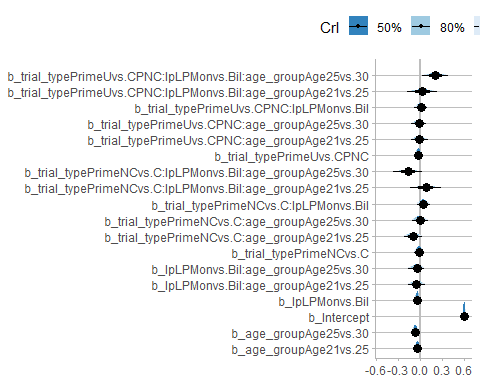
\includegraphics{2021-01-25_lacre_files/figure-latex/unnamed-chunk-2-1.pdf}

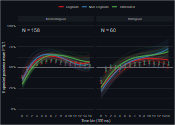
\includegraphics{2021-01-25_lacre_files/figure-latex/gaze_time-1.pdf}

\hypertarget{references}{%
\subsection*{References}\label{references}}
\addcontentsline{toc}{subsection}{References}

\hypertarget{refs}{}
\begin{CSLReferences}{1}{0}
\leavevmode\vadjust pre{\hypertarget{ref-bosch2001evidence}{}}%
Bosch, Laura, and Núria Sebastián-Gallés. 2001. {``Evidence of Early
Language Discrimination Abilities in Infants from Bilingual
Environments.''} \emph{Infancy} 2 (1): 29--49.

\leavevmode\vadjust pre{\hypertarget{ref-bosma2020cognate}{}}%
Bosma, Evelyn, and Naomi Nota. 2020. {``Cognate Facilitation in
Frisian--Dutch Bilingual Children's Sentence Reading: An Eye-Tracking
Study.''} \emph{Journal of Experimental Child Psychology} 189: 104699.

\leavevmode\vadjust pre{\hypertarget{ref-burkner2017brms}{}}%
Bürkner, Paul-Christian. 2017. {``Brms: An r Package for Bayesian
Multilevel Models Using Stan.''} \emph{Journal of Statistical Software}
80 (1): 1--28.

\leavevmode\vadjust pre{\hypertarget{ref-byers2021multilab}{}}%
Byers-Heinlein, Krista, Angeline Sin Mei Tsui, Christina Bergmann,
Alexis K Black, Anna Brown, Maria Julia Carbajal, Samantha Durrant, et
al. 2021. {``A Multilab Study of Bilingual Infants: Exploring the
Preference for Infant-Directed Speech.''} \emph{Advances in Methods and
Practices in Psychological Science} 4 (1): 2515245920974622.

\leavevmode\vadjust pre{\hypertarget{ref-costa2000cognate}{}}%
Costa, Albert, Alfonso Caramazza, and Nuria Sebastian-Galles. 2000.
{``The Cognate Facilitation Effect: Implications for Models of Lexical
Access.''} \emph{Journal of Experimental Psychology: Learning, Memory,
and Cognition} 26 (5): 1283.

\leavevmode\vadjust pre{\hypertarget{ref-mani2010infant}{}}%
Mani, Nivedita, and Kim Plunkett. 2010. {``In the Infant's Mind's Ear:
Evidence for Implicit Naming in 18-Month-Olds.''} \emph{Psychological
Science} 21 (7): 908--13.

\leavevmode\vadjust pre{\hypertarget{ref-mani2011phonological}{}}%
---------. 2011. {``Phonological Priming and Cohort Effects in
Toddlers.''} \emph{Cognition} 121 (2): 196--206.

\leavevmode\vadjust pre{\hypertarget{ref-mirman2017growth}{}}%
Mirman, Daniel. 2017. \emph{Growth Curve Analysis and Visualization
Using r}. Chapman; Hall/CRC.

\leavevmode\vadjust pre{\hypertarget{ref-thierry2007brain}{}}%
Thierry, Guillaume, and Yan Jing Wu. 2007. {``Brain Potentials Reveal
Unconscious Translation During Foreign-Language Comprehension.''}
\emph{Proceedings of the National Academy of Sciences} 104 (30):
12530--35.

\leavevmode\vadjust pre{\hypertarget{ref-von2012language}{}}%
Von Holzen, Katie, and Nivedita Mani. 2012. {``Language Nonselective
Lexical Access in Bilingual Toddlers.''} \emph{Journal of Experimental
Child Psychology} 113 (4): 569--86.

\end{CSLReferences}

\end{document}
